%!TEX root = ../thesis.tex

\chapter{Supplementary theory}
\label{ch:theory}

\section{Solar Home System}
Solar home systems exist in various different sizes to address different needs. Common for them all are that they are stand-alone systems, designed to be implemented into a single household. Not being attached to the grid, their main purpose is to generate and store enough electricity during the daylight. Hopefully storing enough energy in the batteries to power lights or other appliances until the next light comes again. This cycle is demonstrated in figure \ref{fig:SHS_drawing}.

\begin{figure}[h]
    \centering
    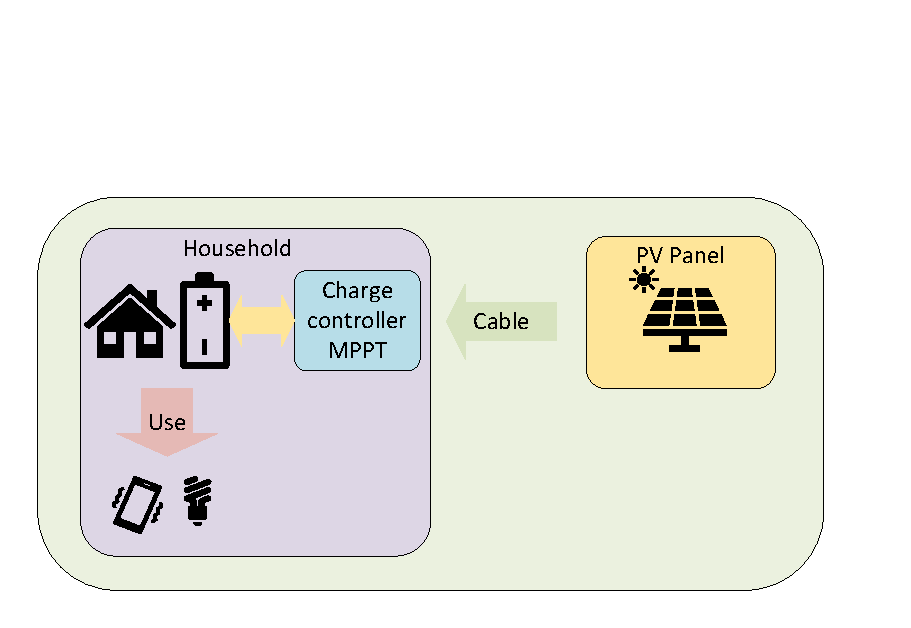
\includegraphics[width=\linewidth]{photos/SHS_drawing.pdf}
    \caption{Solar Home System connection}
    \label{fig:SHS_drawing}
\end{figure}

The PV panel will provide a voltage to the charge controller, which will charge battery. The battery will then supply low power appliances like phones and lights. 

To perform optimal charging, a \acrfull{mppt} controller is used. The controller finds the optimal voltage to current ratio for charging based on the voltage from the PV panel. This ensures optimal charging even when the PV panel does not have optimal conditions, such as shading, low sun or dirt on the panel.

\subsection{Power generation}

\subsubsection{Photovoltaic}
For photovoltaic cells to capture energy from light sources, they need to absorb photons into their silicon wafer. When a photon is absorbed in silicon, its energy is transferred to an electron. This process is what makes it possible to transform light into usable electric charge. How many photons that enter this wafer is what decides how much energy the PV module will capture. Factors like irradiance, angle and temperature change how many photons get absorbed \citep{wirthPhotovoltaicModulesTechnology2016}.

\subsubsection{Irradiance}
The number of photons that hit an area\footnote{Called the quantum flux}, will decide the amount of irradiance. Irradiance will rise during a day, ending up with being strongest when the angle of the sun is perpendicular to the surface it shines against. Since the angle the sun will have on the earth changes during the year, the actual irradiance will also change correspondingly. Affecting parts further from equator more than those closer, seasonal variations will increase or reduce daily irradiance. Light will scatter more in a low hanging winter sun than when given a long lasting summer sun. Weather variations will also change the way light scatters. Cloudy weather will give a reduced amount of irradiance, while clear low humidity weather will give more irradiance. 

To estimate irradiance, we can use formulas or simulations. These being created on the angle of the sun and weather variations, we can find an accurate representation of the actual conditions. 

\subsubsection{Solar panel}
Solar panels will have a wattage peak effect, limiting how much energy they can absorb in the solar cells. Larger panels will absorb more sunlight, creating more electricity. To account for the direction of the sun, having an angle on the solar panel will give an increased irradiance.

Solar panels have varying amount of loss, but one way of analyzing the performance ratio of the module is equation \eqref{eq:performanceratio}.

\begin{align}
    PR_{mod} & = \frac{E_{DC}}{H_{POA}A_{MOD}\eta_{STC}}
    \label{eq:performanceratio}
\end{align}
Where:
\begin{itemize}
    \item $PR_{MOD}$ is annual module performance ratio
    \item $E_{DC}$ is annual som of delivered energy assuming MPPT $[MJ]$
    \item $H_{POA}$ is annual irradiation into plane of the module $[MJ/m^2]$
    \item $A_{MOD}$ is total module area $[m^2]$
    \item $\eta_{STC}$ is module efficiency under standard test conditions (STC).
\end{itemize}

To find this, we need to know the performance module efficiency. This is measured during standard conditions of 1000 $W/m^2$ and \SI{25}{\celsius}. See equation \eqref{eq:panelefficiency}

\begin{align}
    \eta_{mod} &= \frac{P_{mod}}{E_{STC}A_{mod}}
    \label{eq:panelefficiency}
\end{align}
Where:
\begin{itemize}
    \item $\eta_{mod}$ is the module efficiency
    \item $P_{MOD}$ is maximum power point
    \item $E_{STC}$ is irradiance at standard test conditions
    \item $A_{MOD}$ is total module area $[m^2]$
\end{itemize}

\subsubsection{Soiling}
Soiling on the panel will cover the modules, hindering photon absorption and reducing module efficiency. Soiling can come from several pollutants such as ash, stone dust, sand, coal powder or cement. Panels get more contaminated based on how much upward-facing surface it has. Equation \eqref{eq:dustreduction} shows the relationship between the tilt angle and the upward-facing surface based on \citep{yakubuHolisticReviewEffects2025}.

\begin{align}
    St & = A \cdot \cos{\alpha}
    \label{eq:dustreduction}
\end{align}
Where:
\begin{itemize}
    \item $St$ is the upward-facing surface
    \item $A$ is the module area 
    \item $\alpha$ is the tilt angle
\end{itemize}
\citep{yakubuHolisticReviewEffects2025} found soiling to reduce the effect from 10\% in mild regions, up to 40\% in arid regions. Manual cleaning showed to restore up to 98\% of the module efficiency. 

\subsubsection{Tilt angle and Azimuth}
When using fixed tilt\footnote{The alternative to fixed tilt is solar tracking, where the panel will adjust itself in coordination with the sun.}, the panel should face the south when in the northern hemisphere. \citep{SolarEnergyEngineering2024} shows that for maximum annual production, the optimal tilt angle can be found using equation \eqref{eq:tiltangle}

\begin{align}
    \alpha & = 0.764L \ + \ 2.14^\circ, for \ L \leq \ 65^\circ
    \label{eq:tiltangle}
\end{align}
Where:
\begin{itemize}
    \item $L$ is the latitude
    \item $\alpha$ is the tilt angle
\end{itemize}

\citep{SolarEnergyEngineering2024} also proposes adjusting for afternoon sun, when the demand is higher. This would mean adjusting the angle higher to capture a low afternoon sun. For a SHS, this can make sense when wanting it fully charged for the night. 

Another factor is the azimuth\footnote{Azimuth is the horizontal angle of a cardinal direction, often south or north. In this case, we use the PVGIS definition of \SI{0}{\degree} azimuth to be south.} of the panel. The most common angle in the northern hemisphere is to use \SI{0}{\degree}, although you can apply the same principle of adjusting for afternoon sun here as well. Fixing the azimuth more towards the setting sun on the east would give more irradiance from a setting sun. This will unfortunately greatly affect production during peak-hours.
\subsection{Battery}

\subsubsection{State of Health}
A battery's \acrfull{soh} will give an indication of how effective a battery is based on how much charge it can hold compared to a nominal charge. The SoH will be reduced by during the lifetime of the battery. Time, high or low temperature, high or low voltage and high current rate will degrade the SoH\citep{liuDataScienceBasedFullLifespan2022}. To find the SoH of a battery, we can use equation \eqref{eq:soh}. This equation will give us two ways to measure the SoH, either using the charge or using the internal resistance. 

\begin{align}
    SoH_{C} &= \frac{C_a}{C_n} \cdot 100\%  \\
    SoH_R &= \frac{R_a - R_r}{R_r} \cdot 100\% 
    \label{eq:soh}
\end{align}
Where:
\begin{itemize}
    \item $C_a$ is actual charge
    \item $C_n$ is nominal charge
    \item $R_a$ is actual internal resistance
    \item $R_r$ is rated internal resistance
\end{itemize}

To find the actual internal resistance, we can apply a known load to the battery and measure before and after the load is applied. This will give us the voltage split over the two resistances, and using ohms law we can find the internal resistance of the battery. 

\subsubsection{Lifetime}
The type of battery and the conditions it is exposed to determines the lifetime\footnote{The lifetime of a battery is when it reaches 80\% of the initial capacity it had} of the battery. On off-grid PV systems, \citep{wieczorekInfluenceCurrentOffgrid2023} found \acrfull{lfp} batteries to be the most lasting when given incomplete charges. In the worst cases having a lead-acid battery last for 30 cycles before reaching it's end of life. 
\subsection{Consumption}

\subsubsection{LED}
\acrfull{led} is a light technology that consumes less energy per lumen than incandescent light bulbs. \citep{usdepartmentofenergyLifeCycleAssessmentEnergy2012} claiming that LED is about one quarter of the energy consumption of incandescent lights per functional unit\footnote{Functional unit is defined as 20 million lumen hours}. The evaluation was done as a life cycle assessment, meaning they looked at the entire process and not just compared power rating and lumen. In terms of lumen per energy unit, \citep{podeLightEmittingDiodes2011} claim LED saves 80\% energy compared to incandescent lighting. 

\subsubsection{Charge port}
\acrfull{usba} is a general interface that is normal for power transfer on phones and other small devices. The standard voltage transfer is 5V, and reaches up to 900mA \citep{jimmylinGettingBottomUSB2021}.

\section{Economic metrics}
\subsection{Levelized cost of energy}
\acrfull{lcoe} is used as a benchmark to determine the cost-effectiveness of different energy generation technologies\citep{brankerReviewSolarPhotovoltaic2011}. The metric uses the lifetime of the equipment, it's cost and the generated energy to estimate a price per unit of energy. The formula of LCOE is show in equation \eqref{eq:LCOEfirst}, which is an expansion of the \acrfull{npv} calculation. When using NPV we also need to introduce a discount rate for the investment and income.

\begin{align}
    LCOE & = \frac{NPV(Costs)}{NPV(EnergyIncome)} \notag \\
    \notag \\
    LCOE &= \frac{\Sigma_{t=0}^T  C_t/(1+r)^t}{\Sigma_{t=0}^T  E_t/(1+r)^t}
    \label{eq:LCOEfirst}
\end{align}
Where:
\begin{itemize}
    \item $C_t$ is net cost of system for t
    \item $E_t$ is energy produced for t in monetary value
    \item  $r$ is discount rate
    \item $T$ is lifetime of the system
\end{itemize}

When $t=0$ we will have our initial cost included into the net cost of the system. $C_0$ will include both the investment cost and any running costs related to the system. To analyze how worthwhile this investment is, the discount rate needs to be compared to a similar investment and it's expected rate. The calculation of $E_t$ will also be twofold, both the energy yield and the actual energy price. A higher price will give a higher LCOE for the given $t$. Based on the lifetime of the system, we will have a higher LCOE as long as the running costs are low. 

\subsection{Discount rate}
Typically the discount rate is calculated from a purely economical perspective, but for renewable projects \citep{sarahleeUltimateSocialDiscount2025} suggest using \acrfull{sdr}. These rates include the long term benefits such as the effect the renewable energy has on the environment for future generations. \citep{sarahleeUltimateSocialDiscount2025} refers to Ramsey Formula to calculate the SDR, here given in equation \eqref{eq:ramseyformula}.

\begin{align}
    r & = \delta + \eta g
    \label{eq:ramseyformula}
\end{align}
Where:
\begin{itemize}
    \item $r$ is the discount rate
    \item $\delta$ is the pure time preference
    \item  $\eta$ is the elasticity of marginal utility of consumption
    \item  $g$ is the growth rate of per capita consumption
\end{itemize}


\subsection{Life cycle cost}
Similar to LCOE, \acrfull{lcc} will analyze the cost of the system for it's lifetime. The difference is that it will not look at the yield of energy, and only focus of the cost of the product\citep{tonioloLifeCycleThinking2020}. \acrshort{lcc} can be used for a simple analysis of the product in terms of initial purchase, or it could take into account the cost of design, production, transport and end life\citep{tonioloLifeCycleThinking2020}. This means we have to decide what is right for this project to apply the method of \acrshort{lcc}. The conventional method to apply \acrshort{lcc} is to assess all the costs during the life cycle of the product\citep{tonioloLifeCycleThinking2020}. Not being structured by an \acrfull{iso} procedure, the method for calculating the \acrshort{lcc} is subject to interpretation and does not have a specific equation. 


\subsection{Payback time}
Payback time is how long it will take accumulated annual revenue to be equal to the initial investment. This is a simple way to calculate how long it will take for a project to be profitable without including any internal rate of return\citep{dahlquistPrinciplesFinance2022}. This is show in equation \eqref{eq:payback}.

\begin{align}
    Payback\ Period = \frac{IC}{R_n}
    \label{eq:payback}
\end{align}
Where:
\begin{itemize}
    \item $IC$ is initial cost at first year
    \item $R_n$ is annual revenue stream for any year
\end{itemize}

The payback period does not take into account any maintenance costs or end of life costs of the investment. Although to fix this, we can incorporate the costs using only marginal revenue as revenue. As there is no expected costs with the SHS, we will assume that revenue will be equal to marginal revenue.  


